\let\negmedspace\undefined
\let\negthickspace\undefined
\documentclass[journal]{IEEEtran}
\usepackage[a4paper, margin=10mm, onecolumn]{geometry}
\usepackage{lmodern} % Ensure lmodern is loaded for pdflatex
\usepackage{tfrupee} % Include tfrupee package

\setlength{\headheight}{1cm} % Set the height of the header box
\setlength{\headsep}{0mm}  % Set the distance between the header box and the top of the text

\usepackage{gvv-book}
\usepackage{gvv}
\usepackage{cite}
\usepackage{amsmath,amssymb,amsfonts,amsthm}
\usepackage{algorithmic}
\usepackage{graphicx}
\usepackage{float}
\usepackage{textcomp}
\usepackage{xcolor}
\usepackage{txfonts}
\usepackage{listings}
\usepackage{enumitem}
\usepackage{mathtools}
\usepackage{gensymb}
\usepackage{comment}
\usepackage[breaklinks=true]{hyperref}
\usepackage{tkz-euclide} 
\usepackage{listings}
% \usepackage{gvv}                                        
\def\inputGnumericTable{}                                 
\usepackage[latin1]{inputenc}                                
\usepackage{color}                                            
\usepackage{array}                                            
\usepackage{longtable}                                       
\usepackage{calc}                                             
\usepackage{multirow}                                         
\usepackage{hhline}                                           
\usepackage{ifthen}                                           
\usepackage{lscape}
\usepackage{tikz}
\usetikzlibrary{patterns}

\begin{document}

\bibliographystyle{IEEEtran}
\vspace{3cm}

\title{11.2.5}
\author{EE25BTECH11064 - Yojit Manral}

\maketitle
% \maketitle
% \newpage
% \bigskip
{\let\newpage\relax\maketitle}
\renewcommand{\thefigure}{\theenumi}
\renewcommand{\thetable}{\theenumi}
\setlength{\intextsep}{10pt} % Space between text and float

\textbf{Question:}\\
In $\triangle ABC$, $\vec{D}$, $\vec{E}$ and $\vec{F}$ are, respectively, the mid-points of sides AB, BC and CA. Show that $\triangle ABC$ is divided into four congruent triangles by joining $\vec{D}$, $\vec{E}$, and $\vec{F}$.

\textbf{Solution:}\\
$\rightarrow$ Given that
\begin{align}
    \vec{D} = \frac{\vec{A}+\vec{B}}{2} && \vec{E} = \frac{\vec{B}+\vec{C}}{2} && \vec{F} = \frac{\vec{C}+\vec{A}}{2}
\end{align}
$\rightarrow$ From (1), it follows that
\begin{align}
    \vec{A} = \vec{D}+\vec{F}-\vec{E} && \vec{B} = \vec{E}+\vec{D}-\vec{F} && \vec{C} = \vec{F}+\vec{E}-\vec{D}
\end{align}
$\rightarrow$ From (2), we get that
\begin{align}
    \text{In }\triangle FAD\text{ and }\triangle DEF && \text{In }\triangle DBE\text{ and }\triangle DEF && \text{In }\triangle ECF\text{ and }\triangle DEF \\
    \vec{A}-\vec{D} = \vec{F}-\vec{E}\text{ (Side 1)} && \vec{B}-\vec{E} = \vec{D}-\vec{F}\text{ (Side 1)} && \vec{C}-\vec{F} = \vec{E}-\vec{D}\text{ (Side 1)} \\
    \vec{A}-\vec{F} = \vec{D}-\vec{E}\text{ (Side 2)} && \vec{B}-\vec{D} = \vec{E}-\vec{F}\text{ (Side 2)} && \vec{C}-\vec{E} = \vec{F}-\vec{D}\text{ (Side 2)} \\
    \vec{D}-\vec{F}\text{ is common to both} && \vec{E}-\vec{D}\text{ is common to both} && \vec{F}-\vec{E}\text{ is common to both} \\
    \triangle FAD \cong \triangle DEF\text{(SSS criterion)} && \triangle DBE \cong \triangle DEF\text{(SSS criterion)} &&
    \triangle ECF \cong \triangle DEF\text{(SSS criterion)}
\end{align}
$\rightarrow$ From (7), we know that $\triangle ABC$ is divided into four congruent triangles
\begin{align}
    \triangle FAD \cong \triangle DBE \cong \triangle ECF \cong \triangle DEF
\end{align}
\begin{figure}[h!]
   \centering
   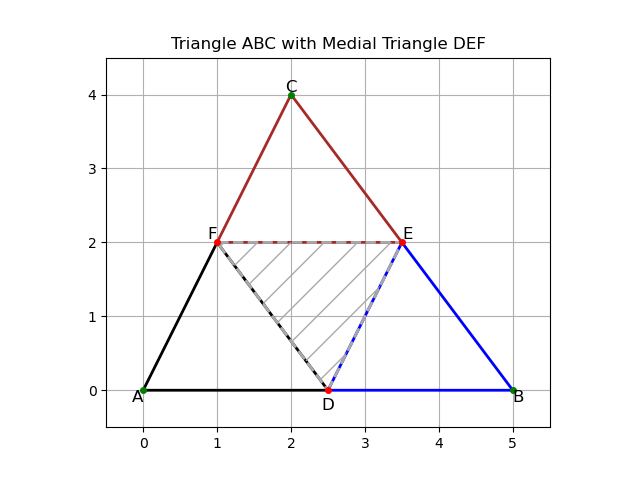
\includegraphics[width=\linewidth]{figs/01.png}
   \caption{Plot of $\triangle ABC$ and its medial triangle $\triangle DEF$}
   \label{Plot_1}
\end{figure}
\end{document}
